
Evaluating the performance of a poker player is a challenging task. Unfortunately, the majority of strong AI poker players are not publicly available. Furthermore, conducting a big-scale experiment against human players is also not feasible, as the big online poker-playing sites prohibit the use of bots. To get an idea of the performance of PokerShark, we conducted a number of experiments where PokerShark played against dummy-AI player and human players. 

\subsection*{Playing against Dummy-AI players}
Dummy-AI players are AI players that use a simple static strategy to play poker. We used four such players: Bold, Fish, Honest and Random. The bold player always raises the maximum allowed amount regardless of his pocket. Similarly, the fish player always calls, whereas the honest player chooses the best action based on the estimated strength of his hand; finally, the random player chooses a random action.
At first glance, one might overlook the challenges imposed by these simple strategies. However, playing against these bots will provide a good chance to see how PokerShark will identify and exploit the weaknesses of each bot.


\subsubsection{Bold Player}
The bold player imposes an interesting problem because the bot will start each round by betting the entire stack; calling such a bet is very risky from the preflop. Looking at the graph shown in figure \ref{fig:results_bold}, we can see that most losses occur before the showdown because PokerShark is folding many weak hands. Although it is a very difficult challenge, PokerShark lost only 0.71 small blinds per hand. This is a very good result, considering that the bold player is a very loose and aggressive player.

\begin{figure}[H]
    \centering
    \begin{minipage}{\textwidth}
        \begin{minipage}{0.40\textwidth}
            \begin{tabular}{|l|l|l|}
                \hline
                \textbf{Number of games}  & 100   &        \\ \hline
                \textbf{Games won}        & 38    & 38.0\% \\ \hline
                \textbf{Games drew}       & 0     & 00.0\%  \\ \hline
                \textbf{Games lost}       & 62    & 62.0\% \\ \hline
                \textbf{Number of rounds} & 3237  &        \\ \hline
                \textbf{Rounds won}       & 110   & 30.4\%  \\ \hline
                \textbf{Rounds drew}      & 0     & 00.0\%  \\ \hline
                \textbf{Rounds lost}      & 3127  & 96.6\% \\ \hline
                \textbf{WPH}              & -0.71 &        \\ \hline
            \end{tabular}
        \end{minipage}
        \hspace{0.05\textwidth}
        \begin{minipage}{0.5\textwidth}
            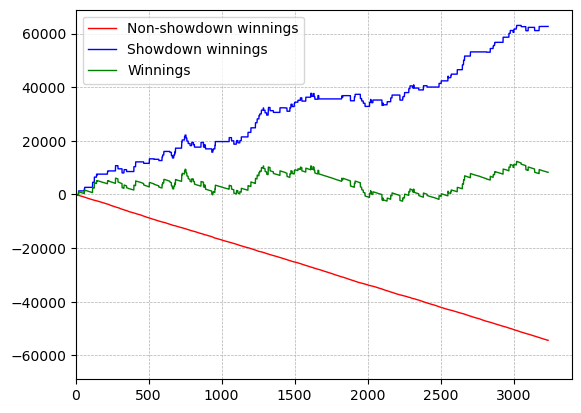
\includegraphics[width=\textwidth]{graphics/bold.png}
        \end{minipage}
    \end{minipage}
    \caption{Results of playing 100 games against the Bold player.}
    \label{fig:results_bold}
\end{figure}

\subsubsection{Fish Player}
Playing against the fish player is a good opportunity to showcase PokerShark's ability to exploit players' tendencies. For example, we can see that PokerShark did not fold as much, meaning it has adjusted its folding range. We can also see that although PokerShark is calling/raising a lot more, it manages the risk by using small raises.

\begin{figure}[H]
    \centering
    \begin{minipage}{\textwidth}
        \begin{minipage}{0.40\textwidth}
            \begin{tabular}{|l|l|l|}
                \hline
                \textbf{Number of games}  & 100  &        \\ \hline
                \textbf{Games won}        & 68   & 68.0\% \\ \hline
                \textbf{Games drew}       & 0    & 00.0\%  \\ \hline
                \textbf{Games lost}       & 32   & 32.0\% \\ \hline
                \textbf{Number of rounds} & 3385 &        \\ \hline
                \textbf{Rounds won}       & 1511 & 44.6\% \\ \hline
                \textbf{Rounds drew}      & 21   & 00.6\%  \\ \hline
                \textbf{Rounds lost}      & 1853 & 54.7\% \\ \hline
                \textbf{WPH}              & 1.10 &        \\ \hline
            \end{tabular}
        \end{minipage}
        \hspace{0.05\textwidth}
        \begin{minipage}{0.5\textwidth}
            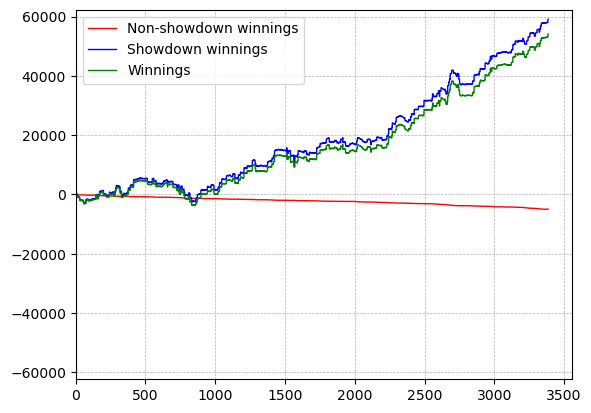
\includegraphics[width=\textwidth]{graphics/fish.png}
        \end{minipage}
    \end{minipage}
    \caption{Results of playing 100 games against the Fish player.}
\end{figure}


\subsubsection{Honest Player}
Playing against a player that does not bluff is quite difficult because it folds when his hand is weak, and he only raises with a strong hand. Therefore, knowing when to challenge such a player is crucial to winning the game. We think PokerShark performed well against this player.
\begin{figure}[H]
    \centering
    \begin{minipage}{\textwidth}
        \begin{minipage}{0.40\textwidth}
            \begin{tabular}{|l|l|l|}
                \hline
                \textbf{Number of games}  & 100   &        \\ \hline
                \textbf{Games won}        & 17    & 17.0\% \\ \hline
                \textbf{Games drew}       & 0     & 00.0\%  \\ \hline
                \textbf{Games lost}       & 83    & 83.0\% \\ \hline
                \textbf{Number of rounds} & 9340  &        \\ \hline
                \textbf{Rounds won}       & 3670  & 39.3\% \\ \hline
                \textbf{Rounds drew}      & 3     & 00.6\%  \\ \hline
                \textbf{Rounds lost}      & 5667  & 60.7\% \\ \hline
                \textbf{WPH}              & -0.16 &        \\ \hline
            \end{tabular}
        \end{minipage}
        \hspace{0.05\textwidth}
        \begin{minipage}{0.5\textwidth}
            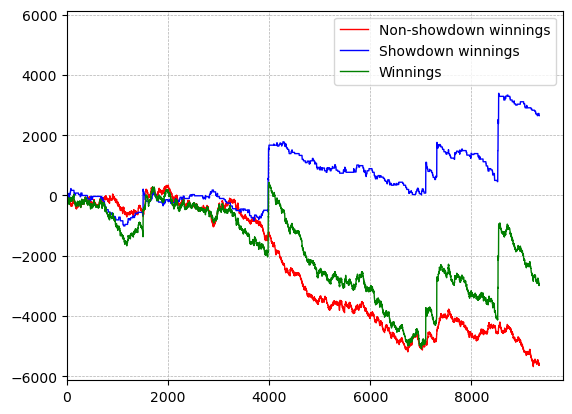
\includegraphics[width=\textwidth]{graphics/honest.png}
        \end{minipage}
    \end{minipage}
    \caption{Results of playing 100 games against the Honest player.}
\end{figure}


\subsubsection{Random Player}
Facing a random opponent is a great way to see how PokerShark handles contradictory information while modeling its opponent. The graph shows PokerShark used bigger betting amounts while also folding more often. 

\begin{figure}[H]
    \centering
    \begin{minipage}{\textwidth}
        \begin{minipage}{0.40\textwidth}
            \begin{tabular}{|l|l|l|}
                \hline
                \textbf{Number of games}  & 100   &        \\ \hline
                \textbf{Games won}        & 48    & 48.0\% \\ \hline
                \textbf{Games drew}       & 0     & 00.0\%  \\ \hline
                \textbf{Games lost}       & 52    & 52.0\% \\ \hline
                \textbf{Number of rounds} & 4540  &        \\ \hline
                \textbf{Rounds won}       & 1276  & 28.1\% \\ \hline
                \textbf{Rounds drew}      & 0     & 00.6\%  \\ \hline
                \textbf{Rounds lost}      & 3264  & 71.9\% \\ \hline
                \textbf{WPH}              & -0.03  &        \\ \hline
            \end{tabular}
        \end{minipage}
        \hspace{0.05\textwidth}
        \begin{minipage}{0.5\textwidth}
            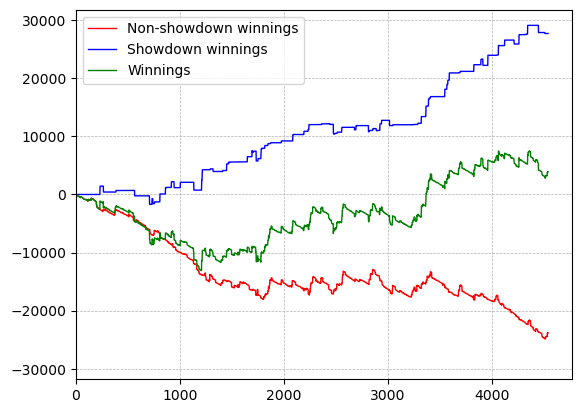
\includegraphics[width=\textwidth]{graphics/random.png}
        \end{minipage}
    \end{minipage}
    \caption{Results of playing 100 games against the Random player.}
\end{figure}

\subsection{Playing against human players}
Unfortunately, we could not organize a big experiment to test PokerShark's performance against human players. However, we were able to organize a few games with novice poker players. In total, PokerShark played a round thousand hands against human players.

\begin{figure}[H]
    \centering
    \begin{minipage}{\textwidth}
        \begin{minipage}{0.40\textwidth}
            \begin{tabular}{|l|l|l|}
                \hline
                \textbf{Number of games}  & 18   &        \\ \hline
                \textbf{Games won}        & 10    & 55.6\% \\ \hline
                \textbf{Games drew}       & 0     & 00.0\%  \\ \hline
                \textbf{Games lost}       & 8    & 44.4\% \\ \hline
                \textbf{Number of rounds} & 955  &        \\ \hline
                \textbf{Rounds won}       & 359  & 37.6\% \\ \hline
                \textbf{Rounds drew}      & 1     & 00.1\%  \\ \hline
                \textbf{Rounds lost}      & 595  & 62.3\% \\ \hline
                \textbf{WPH}              & 0.19  &        \\ \hline
            \end{tabular}
        \end{minipage}
        \hspace{0.05\textwidth}
        \begin{minipage}{0.5\textwidth}
            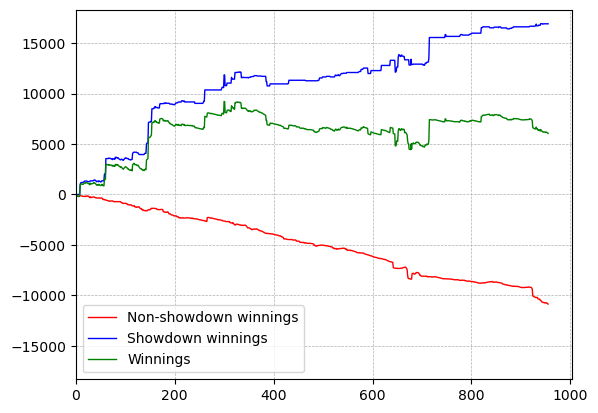
\includegraphics[width=\textwidth]{graphics/human.png}
        \end{minipage}
    \end{minipage}
    \caption{Results of around 1000 hands against human players.}
\end{figure}

Observing the graph, it is clear that PokerShark forfeited a significant portion of its profits by folding. That is due to the majority of human players being able to quickly identify and exploit PokerShark's tendency to fold when calling is too risky. The big fluctuations in winnings indicate that PokerShark did not always fold but was also able to call the opponent's bluff and score big wins.


\section*{Conclusion}
Developing a strong AI poker player involves many challenges, including decision-making under uncertainty, risk management, game theory, and understanding the behavior and psychology of the opponents. PokerShark succeeded in overcoming some of these challenges resulting in a mediocre poker player with great potential for improvement. The performance of the bot can be significantly enhanced by utilizing other opponent modeling techniques as well as an improved utility function. Nevertheless, the purpose of this study was not to create the best poker player but to study how HTN planning would perform in a complex domain such as poker.

Although PokerShark is only a modest poker player, we believe it accomplishes its task as it proves that utilizing HTN planning with risk awareness is a great tool and a strong foundation that is suitable for developing a powerful autonomous agent that can play poker efficiently.

